\documentclass[tikz,border=2mm]{standalone}
\usepackage{lmodern}

\usetikzlibrary{positioning, backgrounds, fit, shapes.arrows}

\begin{document}
	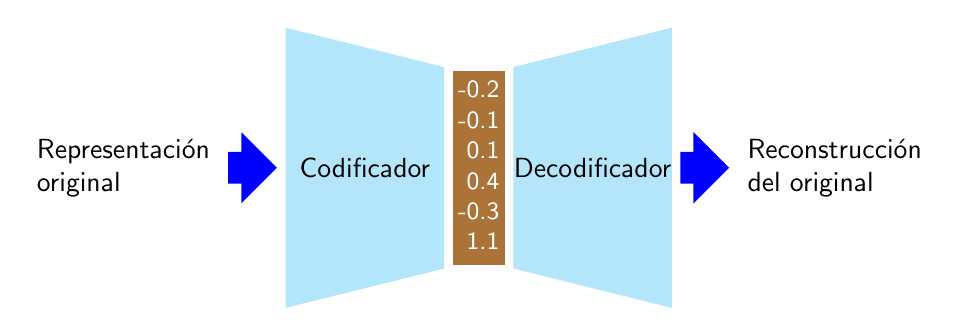
\begin{tikzpicture}[font=\sffamily]
		\node[fill=brown!90!black, text=white, font=\sffamily\small, inner sep=2pt] (a) {\begin{tabular}{@{}r@{}}-0.2\\-0.1\\0.1\\0.4\\-0.3\\1.1\end{tabular}};
		
		\node[fit=(a.north) (a.south), inner sep=1pt, right=1mm of a, minimum width=2cm, label=center:Decodificador] (dec) {};
		\node[fit=(a.north) (a.south), inner sep=1pt, left=1mm of a, minimum width=2cm, label=center:Codificador] (enc) {};
		
		\begin{scope}[on background layer]
			\fill[cyan!30] (dec.north west)--([yshift=5mm]dec.north east)--([yshift=-5mm]dec.south east)--(dec.south west)--cycle;
			\fill[cyan!30] (enc.north east)--([yshift=5mm]enc.north west)--([yshift=-5mm]enc.south west)--(enc.south east)--cycle;
		\end{scope}
		
		\node[right=1mm of dec, fill=blue, single arrow] (b) {\phantom{a}};
		\node[align=left, right=1mm of b] {Reconstrucción\\ del original};
		
		\node[left=1mm of enc, fill=blue, single arrow] (c) {\phantom{a}};
		\node[align=left, left=1mm of c] {Representación\\ original};
	\end{tikzpicture}
\end{document}